\subsection*{Nejlepší uďovský zážitek na táboře}
\label{sub:nejlepší_uďovský_zážitek_na_táboře}

Bohužel tento text vzniká přesně 131 dní po konci tábora, což znamená, že zážitky již v paměti nejsou tak živé. Nicméně, sepíšu alespoň sled výrazných událostí, které mě na táboře ovlivnily, a které přece jen ještě v paměti zůstávají.

Nakládáme materiál pro oba tábory náhodně do tranzitů, celý tábor si vozíme věci z jednoho tábořiště do druhého, Příšery si postupně kopají bazény v lese místo later(je tam fakt hodně vody), Urzoni jsou na stavebce, stavíme týpko na 4x, Špuntí šmouloprogram má úspěch, koupeme se o půlnoci v rybníce, král pirátů byl oběšen, Pískleti spadla sekera na hlavu, oholil jsem si vousy a nechal si jen velmi slušivý knír, dostali jsme kurděje a celý den se jí jen zelenina, Urzoni propíchli týpko chlopňovkou, Kámen kamení, během manévrů jachtíme v bezvětří na Orlíku, pozorujeme hvězdy, Jula přepadá tábor, Míček naučila papouška Kukumbrie novým hláškám, přeučujeme papouška na jiné hlášky, není sauna, Karkulka si zabodla dřevo do nohy, jedeme se koupat do Vltavy, holky smaží šílené množství řízků, poslední 2 dny tábora jíme jen řízky, šílené balení/vybalování a návrat z tábora, v Praze je maraton. 

\begin{center}

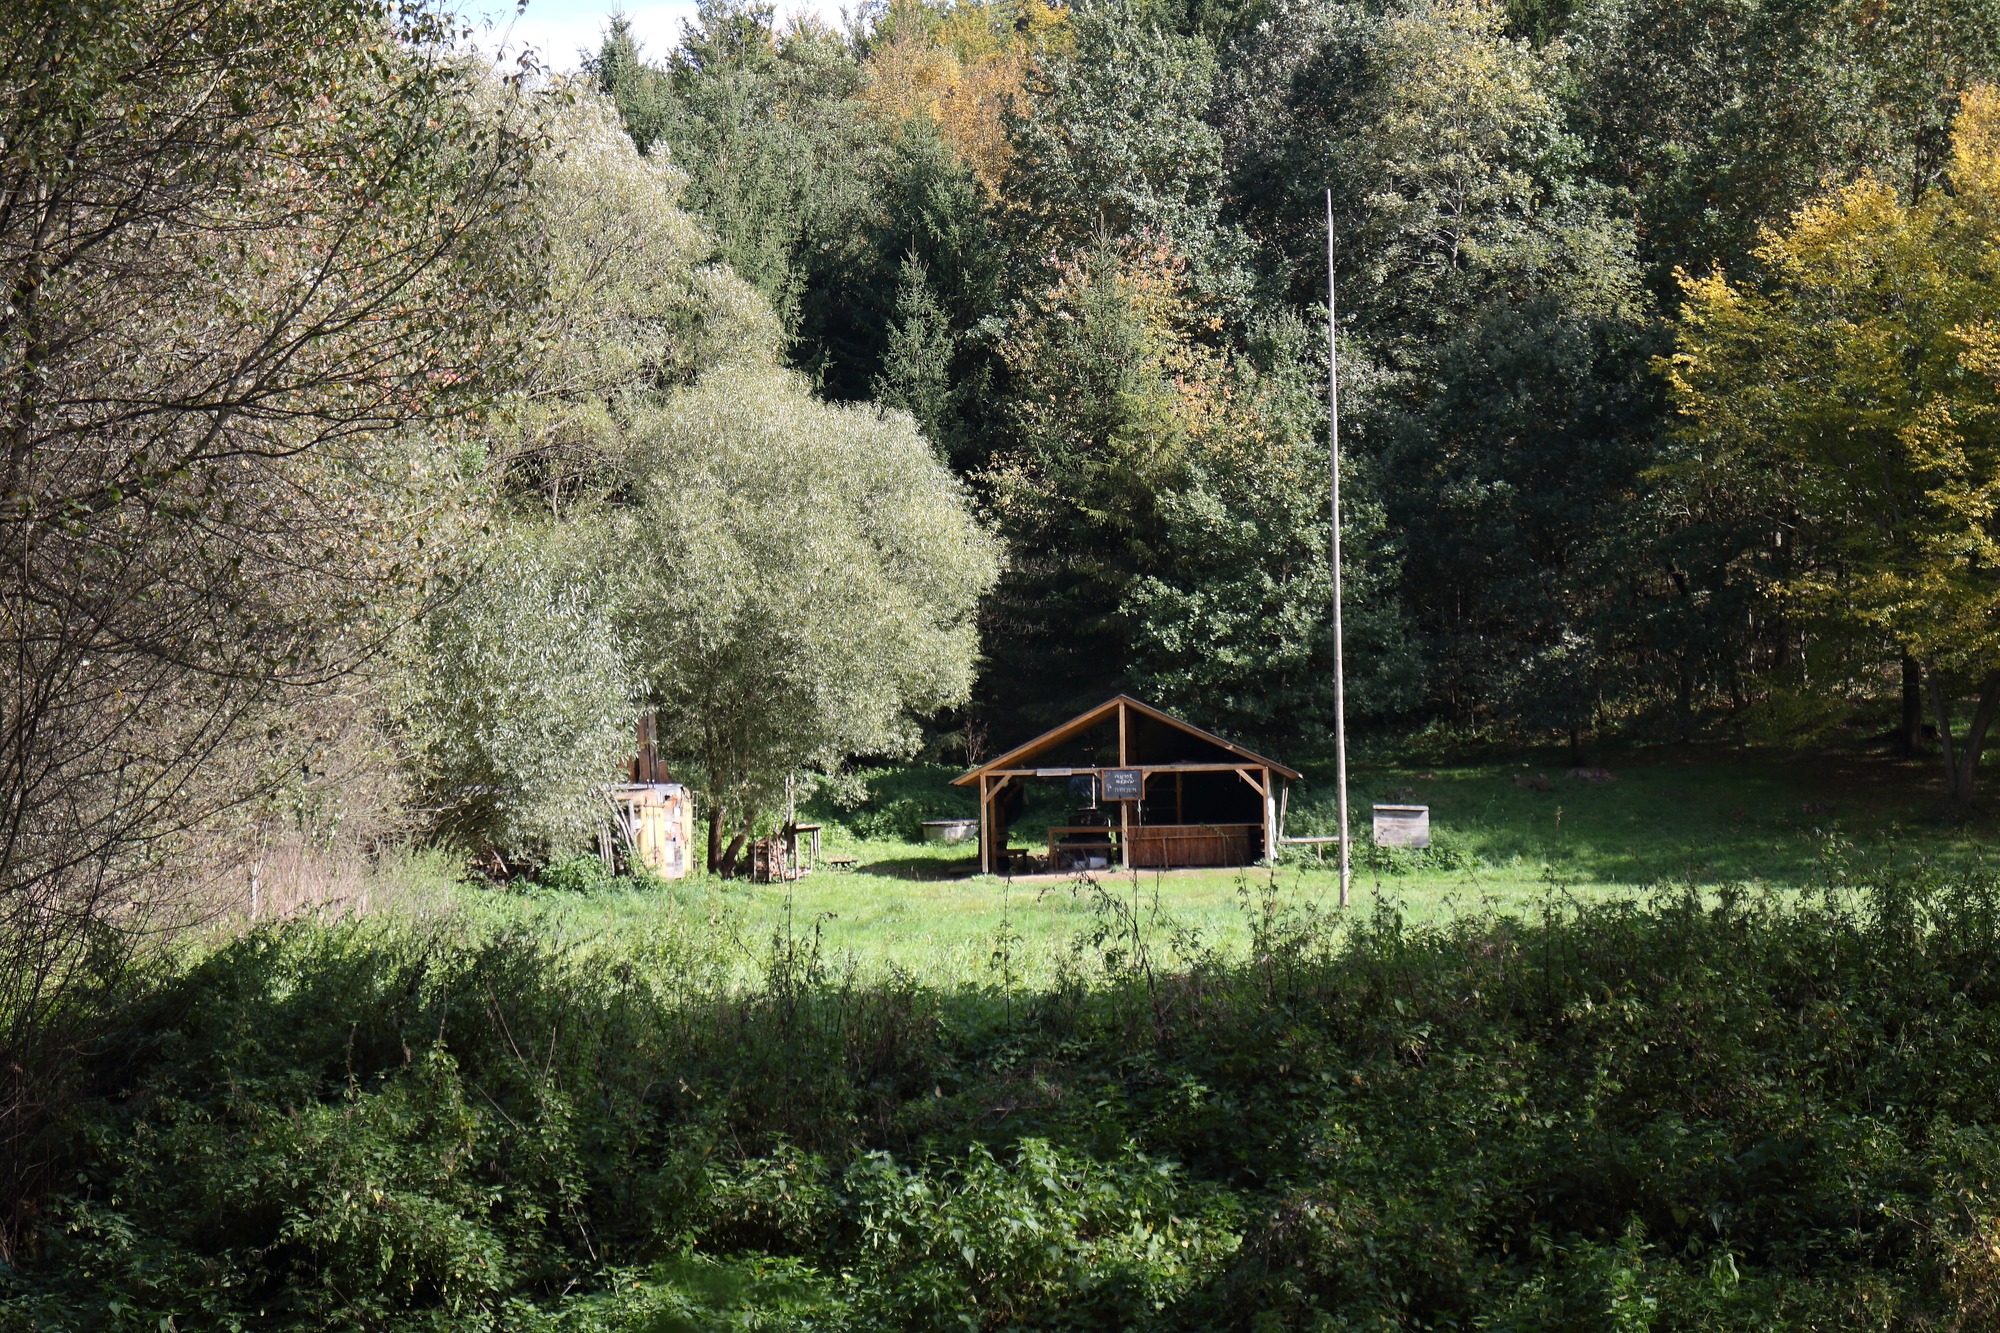
\includegraphics[width=10.2cm]{img/udo_clanky/hledanitaboriste.JPG}

\end{center}

\podpis{Humr}

\clearpage


\subsection *{Omán - země sultána, nafty za 10 korun a pánských pyžam}
\label{sub:omán_-_země sultána_ nafty_za_10_korun_a_pánských_pyžam}

V rámci svého studia na Fildě jsem se vydal na kurz arabštiny do Ománu. Fakulta mi tak umožnila strávit 2 měsíce na Univerzitě Sultána Qábúse pro výuku arabštiny v Manahu – malé vesnici na pomezí Zelených hor a pouště. Studium na Univerzitě zní honosně, ale v Manahu je fakulta specializovaná pouze na výuku arabštiny pro studenty, jejichž rodným jazykem není arabština a tím pádem to je spíše komorní záležitost. Dohromady se nás sešlo 25 nadšenců různých věků a velikostí z celého světa – od Indonésie až po Velkou Británii. 

Nevím, co se vám vybaví, když se řekne Omán. Já každopádně před odletem myslel na vedro, velbloudy a mrakodrapy. Na konci října bylo v Praze okolo 0, Maskat (hlavní město) mě přivítal ve 2 v noci svěžími 30 stupni. Velbloudy tu vídám celkem pravidelně – kus od koleje je velbloudí farma (plot s beduínem a velbloudy) – a mrakodrapy tu nejsou, protože je SQ(sultán Qábús) zakázal – rušily by urbanistický ráz města! 

Jinak ale tato zem, původně zvaná Magan, působí úplně jinak, než jiné arabské státy. \\
Za prvé, všude jsou fotky SQ v různých pózách (sultán Qábús sedící, klečící, mávající, vzdávající se, usmívající se, važný, s holí a s mečem) a vše se tady jmenuje po SQ  - nemocnice, univerzity, školky, mešity, knihovny, lékárny, městské čtvrti - dokonce i na všech bankovkách je jen sultán. Oproti šíleným diktátorům a generálům jinde mají Ománci svého sultána rádi a neustále se usmívají… Také se k tomu váží příjemně časté oslavy narozenin Sultána, státních svátků, narozenin proroka, arabštiny a dalších příležitostných možností k tomu udělat si volno.

Za druhé, díky masivní výstavbě dálnic to tu vypadá jako v USA, akorát místo lánů kukuřice je kamenitá poušť a hory. Jako v USA to tu i funguje – bez auta a klimatizace se daleko nedostanete. Ve škole svádíme neustálý boj s učiteli o mukajjif (větrák), protože místní jsou nadšení z toho, když můžou vychladit místnost pod 20 stupňů. V kombinaci s venkovní teplotou to představuje smrtelné kombo.

Takový běžný Ománec (muž) nosí většinu svého života volné jednodílné pyžamo – říká se mu dišdáša – a je to oblek velmi pohodlný, a však nedá se v něm běhat, sedět nebo klečet – aniž by nebylo třeba ho vykasat. V práci se nosí masar nebo hamdáníja = šátek zavázaný do turbanu. Po práci už jen kumma – kastrolovitá čapka. Mladé Ománky jsou ovlivněné módou ze Zálivu a Saudské Arábie, takže ven vyráží zásadně celé v černém – hidžáb i abája - doma si ale nosí co chtějí. Jakmile jsou již dostatečně staré (bohužel jsem zatím nezjistil přesný věk zlomu – je to něco mezi 30 a smrtí), nosí tradiční, ultranazdobené a barevné oblečení. Vypadají pak jako noční můra všech epileptiků.

Když se Ománci potkají, následuje zhruba 1minutový rituál, během kterého si podají ruce, začnou třást, dotknou se nosem, navzájem se optají, co je nového a navzájem si odpoví, že vůbec nic. Až po rituálu se přejde na věc a můžou si říct, co že je tedy nového. 

Co se týče jídla, místní typická strava se skládá především z rýže, kuřete, datlí, rýže, humusu, datlí, zeleniny s kečupem, rýže, nánů(chlebových placek) a datlí a rýže. Pije se zásadně „šáj karak“, neboli přeslazená silná masala a káva s kardamomem a hřebíčkem. 

Jako všude jinde na Blízkém Východě, i zde si lidé váží nadmíru vody. Ománci jsou náležitě hrdí na svůj 3000 let starý systém „Afládž“ neboli zavlažovací kanály, které jsou zapsány na seznamu UNESCO (nyní vybetonované strouhy). To bohužel ale znamená, že hlavní atrakce veškerých výletů jsou vyschlá vádí, studny a kanály. Historie pevnosti netřeba, hlavně když je afládž…

Univerzita organizuje nejen vyučování, ale i program kulturní – krom návštěvy mnoha pevností (pokud někdy zamíříte do Ománu, stačí vidět jen jednu – např. pevnost Nizwa) jsme zatím například fandili při závodech velbloudů(kvůli vedru se závodí ráno v půl šesté nebo pozdě večer), smlouvali na trzích o věci vyrobené v Číně, oblékali se do tradičního oblečení nebo plavali ve vádí. 

Celkově si vlastně nemůžu stěžovat –starají se tu o mě pěkně, objevuji další kus světa, v rámci kulturní akce jsem se stihl poprvé oženit a trénuju arabštinu – pro studenty obzvlášť výhodné. 

\podpis{Humr}


\subsection*{Převoz tyčí aneb reklama na Boba}
\label{sub:převoz_tyčí_aneb_reklama_na_Boba}

Zajištění tábora je po všech stránkách zajímavá a občas dost náročná záležitost, která se skládá z mnoha dílčích úkolů. Patří mezi ně hledání tábořiště, obvolávání a navštěvování vlastníků, plánování programů a mnoho dalších nutností. Jak už z názvu vyplývá, rád bych vám představil letošní úspěšný převoz.

Vše začíná na Kačerově, kde se scházíme v pátek v podvečer. Vyrážíme ve složení já(Humr a auto), Hafík, Koala a Terka . Dohoda s Bobem zní, že se potkáme s jeho tranzitem na kopci nad tábořištěm Hanyetu u Syrova. Vzhledem k očekávané situaci na dálnici (zprávami zrovna běžely hrůzné zkazky o ucpané D1) se rozhodujeme pro cestu přes Benešov a Vlašim. Cesta z Prahy, která by normálně měla trvat okolo 1 hodiny po dálnici se tak měla o půlhodinky prodloužit. Nápad jet přes Benešov má bohužel víc lidí, takže nakonec dorážíme na místo s 1,5hodinovým zpožděním. Bob se prozíravě rozhodl ignorovat fake news a přijíždí i s vozejkem po dálnici, takže si stíhá užít pěkný západ slunce a začít s taháním týpiovek. Tyče zbyly na tábořišti po zimních týpkařích – šlo jen o jedno týpí – zbytek je uložen na pile u Jiřiček. Za večer stihneme jakž takž vytahat tyče nahoru k autu – kopec bychom nevyjeli – a utábořit se na louce u Jiřiček. Večer se vyrábí večeře ze všech možných zbytků, kombinace nudlí, tortill, Terčina salátu(polníček?) a konzerv je lahodná.

Vstáváme brzy, abychom začali co nejdříve, čeká nás totiž převoz asi 150 kousků do 100 kilometrů vzdálené Vráže. Dle map bude cesta trvat 1,5 hodiny a nejsme si jisti, kolik tyčí zvládneme převézt v jedné várce. Každopádně, doufáme, že se nám podaří vše odvézt během dne, abychom byli večer doma (bláhové?).

Tyčí je mnoho, počítání náročné, 1.várka nám zabrala asi hodinu a čouhá metr a půl přes vozejk (většina tyčí má okolo 9m a více), snad tomu aspoň trochu pomůže červený praporek. Jedou obě vozidla – já s Koalou a Hafíkem se stavíme koupit oběd a potenciální večeři, a Bob s Terkou míří rovnou na tábořiště. Sraz máme ve Vráži u kapličky, s obědem i lahodnými zbytky od večeře čekáme na tyče. Voláme s tranzitem a zjišťujeme, že to vzali přes vesnici, ze které nevede most na druhý břeh Vltavy a teď musí vycouvat zpět na hlavní silnici. Nakonec doráží s mírným zpožděním, vykládáme tyče, necháváme doprovodné vozidlo ve Vráži a jedeme si pro další várku. Cestu si krátíme přednáškami z historie, recitací klasické arabské poezie, vyprávěním příběhů z dávných dob uďovství a debatováním o tématech, které si už nepamatuji, ale pamatuji si, že se o nich velmi živě debatovalo… Jo, a je pekelné vedro. 

Druhá várka nám jde od ruky a vypadá to, že bude náš tyčový park naložen, ale nakonec ještě asi 30 tyčí zbude. Pár tyčí pro jistotu seřízneme, naobědváme se a hurá směr Vráž. Témata pomalu dochází, spánek přichází. Bob naštěstí nespí a řídí. Poslední várku už nějak dotlačíme na vozík, vyfotíme se a odvezeme se. Jsme všichni mrtví a nechápeme, že Bob ještě zvládá řídit. Nu, je to Bob. Končíme v půl osmé po 12 hodinách převážení, nakládání a vykládání. Jdeme se ještě projít po Anpetu tábořišti, kde je všude vysoká tráva, takže se následně vracíme řádně oklíšťováni.
Nakonec nás čeká cesta do Prahy, během které posloucháme klasickou hudbu. 

Během převozu bylo celkem spáleno 90,3 litrů nafty a ujeto 832 km = průměrná spotřeba 10,85l/100km. Statistika namožených svalů a rozsezených zadků není k dispozici.

\podpis{Humr}